The number of events observed in data and in the Standard Model predictions for
a selected set of exclusive signal regions as defined in
\cref{sec:event-selection-1} are reported in \cref{tab:results}. The total
uncertainty of the \gls{sm} predictions range between 2.4\% for EM1 and 9.7\%
for EM10.
\begin{table}[!h]
  \centering
  \resizebox{\linewidth}{!}{\begin{tabular}{lccccc}
    \toprule
    \multicolumn{6}{c}{Analysis Results} \\
    \midrule \midrule
    \textbf{Exclusive Signal Region } & EM2 & EM4 & EM6 & EM8 & EM9 \\
    Observed events (36.1~$\ifb$) & 67475 & 27843 & 2975 & 512 & 223 \\
    \midrule
    SM prediction & $67100 \pm 1400$ & $27640 \pm 610$ & $2825 \pm 78$
                  & $463 \pm 19$ & $213 \pm 9$ \B \\ \cline{2-6}
    $\wenuplusjets$    & $5510 \pm 140$ & $1789 \pm 59$ & $147 \pm 9$
                       & $18 \pm 1$ & $8 \pm 1$ \T \\
    $\wmunuplusjets$   & $6120 \pm 200$ & $2021 \pm 82$ & $173 \pm 9$
                       & $21 \pm 5$ & $11 \pm 1$ \\
    $\wtaunuplusjets$  & $13680 \pm 310$ & $4900 \pm 110$ & $397 \pm 11$
                       & $55 \pm 5$ & $29 \pm 2$ \\
    $\zeeplusjets$     & $0.03 \pm 0$ & $0.02 \pm 0.02$ & $0 \pm 0$
                       & $0 \pm 0$ & $0 \pm 0$ \\
    $\zmumuplusjets$   & $167 \pm 8$ & $36 \pm 2$ & $2 \pm 0.2$
                       & $0.4 \pm 0.1$ & $0.5 \pm 0.1$ \\
    $\ztautauplusjets$ & $185 \pm 6$ & $68 \pm 4$ & $5.1 \pm 0.3$
                       & $0.3 \pm 0.1$ & $0.31 \pm 0.04$ \\
    $\znunuplusjets$   & $37600 \pm 970$ & $17070 \pm 460$ & $1933 \pm 57$
                       & $337 \pm 12$ & $153 \pm 7$ \\
    $t \bar{t}$, single top & $2230 \pm 200$ & $848 \pm 86$ & $43 \pm 6$
                            & $4 \pm 1$ & $1.3 \pm 0.4$ \\
    Diboson & $1327 \pm 90$ & $874 \pm 64$ & $124 \pm 16$
            & $26 \pm 5$ & $10 \pm 2$ \\
    Multijet background & $170 \pm 160$ & $13 \pm 13$ & $1 \pm 1$
                        & $1 \pm 1$ & $0.1 \pm 0.1$ \\
    Non-collision background & $71 \pm 71$ & $18 \pm 18$ & $0 \pm 0$
                             & $0 \pm 0$ & $0 \pm 0$ \\
    \bottomrule
  \end{tabular}}
  \caption{Number of events in the observed data and Standard Model predictions
    in a representative set of signal regions as defined in
    \cref{sec:event-selection-1}. For the \gls{sm} predictions the quoted
    uncertainty includes both statistical and systematic uncertainties.}
  \label{tab:results}
\end{table}
\cref{fig:kfactors} reports the normalization factors applied to the \gls{mc}
predictions obtained from the fit as described in \cref{sec:fit-strategy}. It
can be seen that a multiplicative factor of 1.35 and 0.87 is calculated for the
V + jets and top background respectively. These factors are applied in
\cref{fig:sr_plots} which shows the comparison between the measured
distributions and the Monte Carlo predictions for the $\met$ and leading jet in
signal regions with $\met > 250$~GeV after the fit.
\begin{figure}[!h]
  \centering
  \begin{subfigure}[t]{.48\linewidth}
    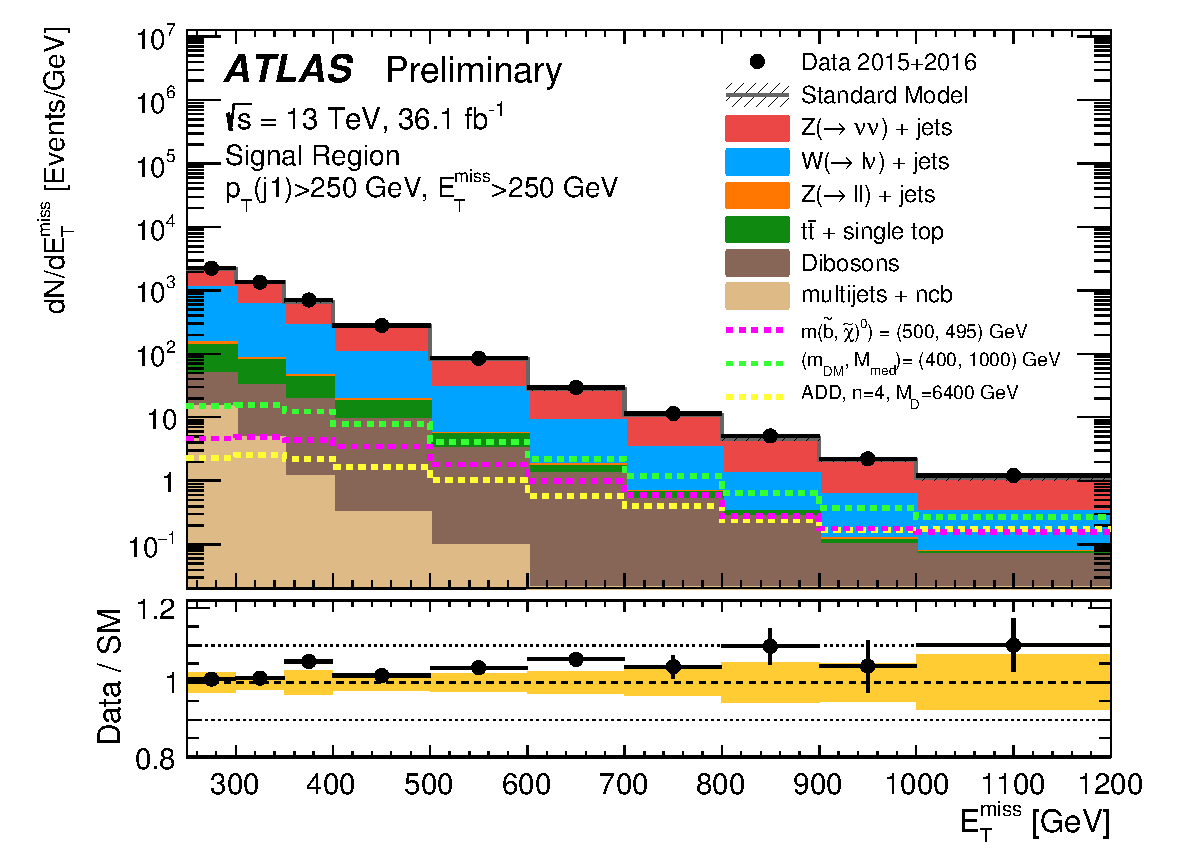
\includegraphics[width=\linewidth]{sr_mod_ind_met}
    \caption{$\met$ distribution.}
    \label{fig:sr_et_miss}
  \end{subfigure}
  \begin{subfigure}[t]{.48\linewidth}
    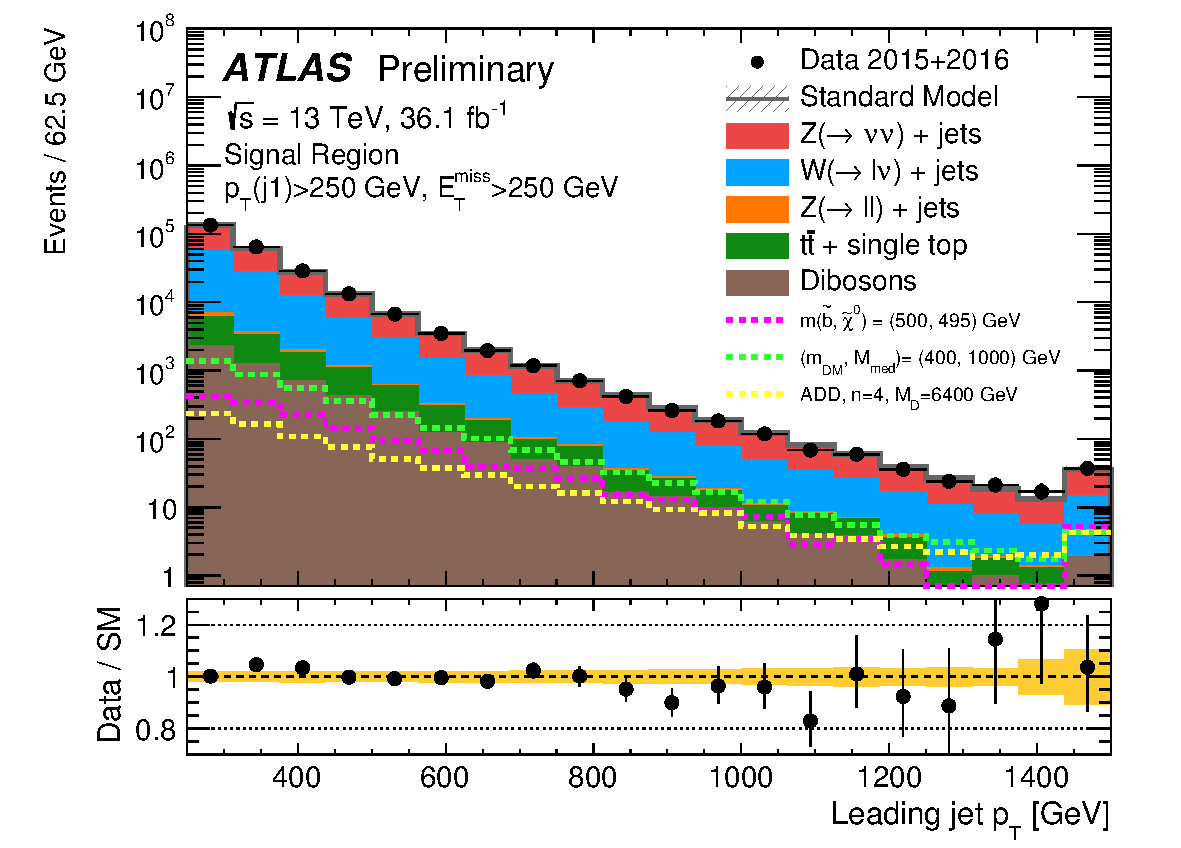
\includegraphics[width=\linewidth]{sr_mod_ind_jetpt}
    \caption{Leading jet $\pt$ distribution.}
    \label{fig:sr_jet1_pt}
  \end{subfigure}
  \caption{Distribution of the $\met$ and the leading jet $\pt$ for IM1 signal
    region compared with the background estimates from the background only fit
    in the control regions. The distributions of different signal models are
    superimposed for comparison. The contribution from the multi-jet and NCB
    background is negligible and not reported in the plot. In the ratio window
    the error bars include experimental and systematic uncertainties.}
  \label{fig:sr_plots}
\end{figure}
\begin{figure}[!h]
  \centering
  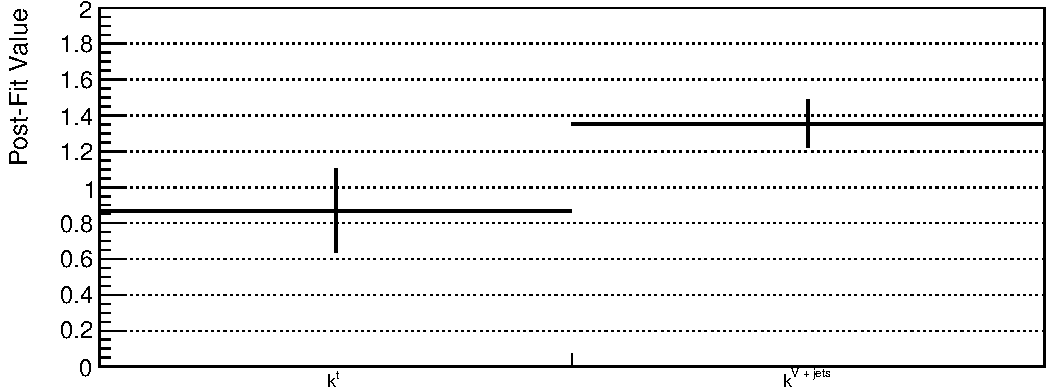
\includegraphics[width=\linewidth]{kfactors}
  \caption{Values of the normalization factors for the V + jets and single top
    backgrounds after the control and signal region inclusive fit to the data.}
  \label{fig:kfactors}
\end{figure}
\cref{fig:np_pull} shows the value of the nuisance parameters defined in
\cref{sec:syst-uncert-1} after the background only fit to the data of the
control and signal regions. In most cases there is a mild constrain of the
parameters.
\begin{figure}[!h]
  \centering
  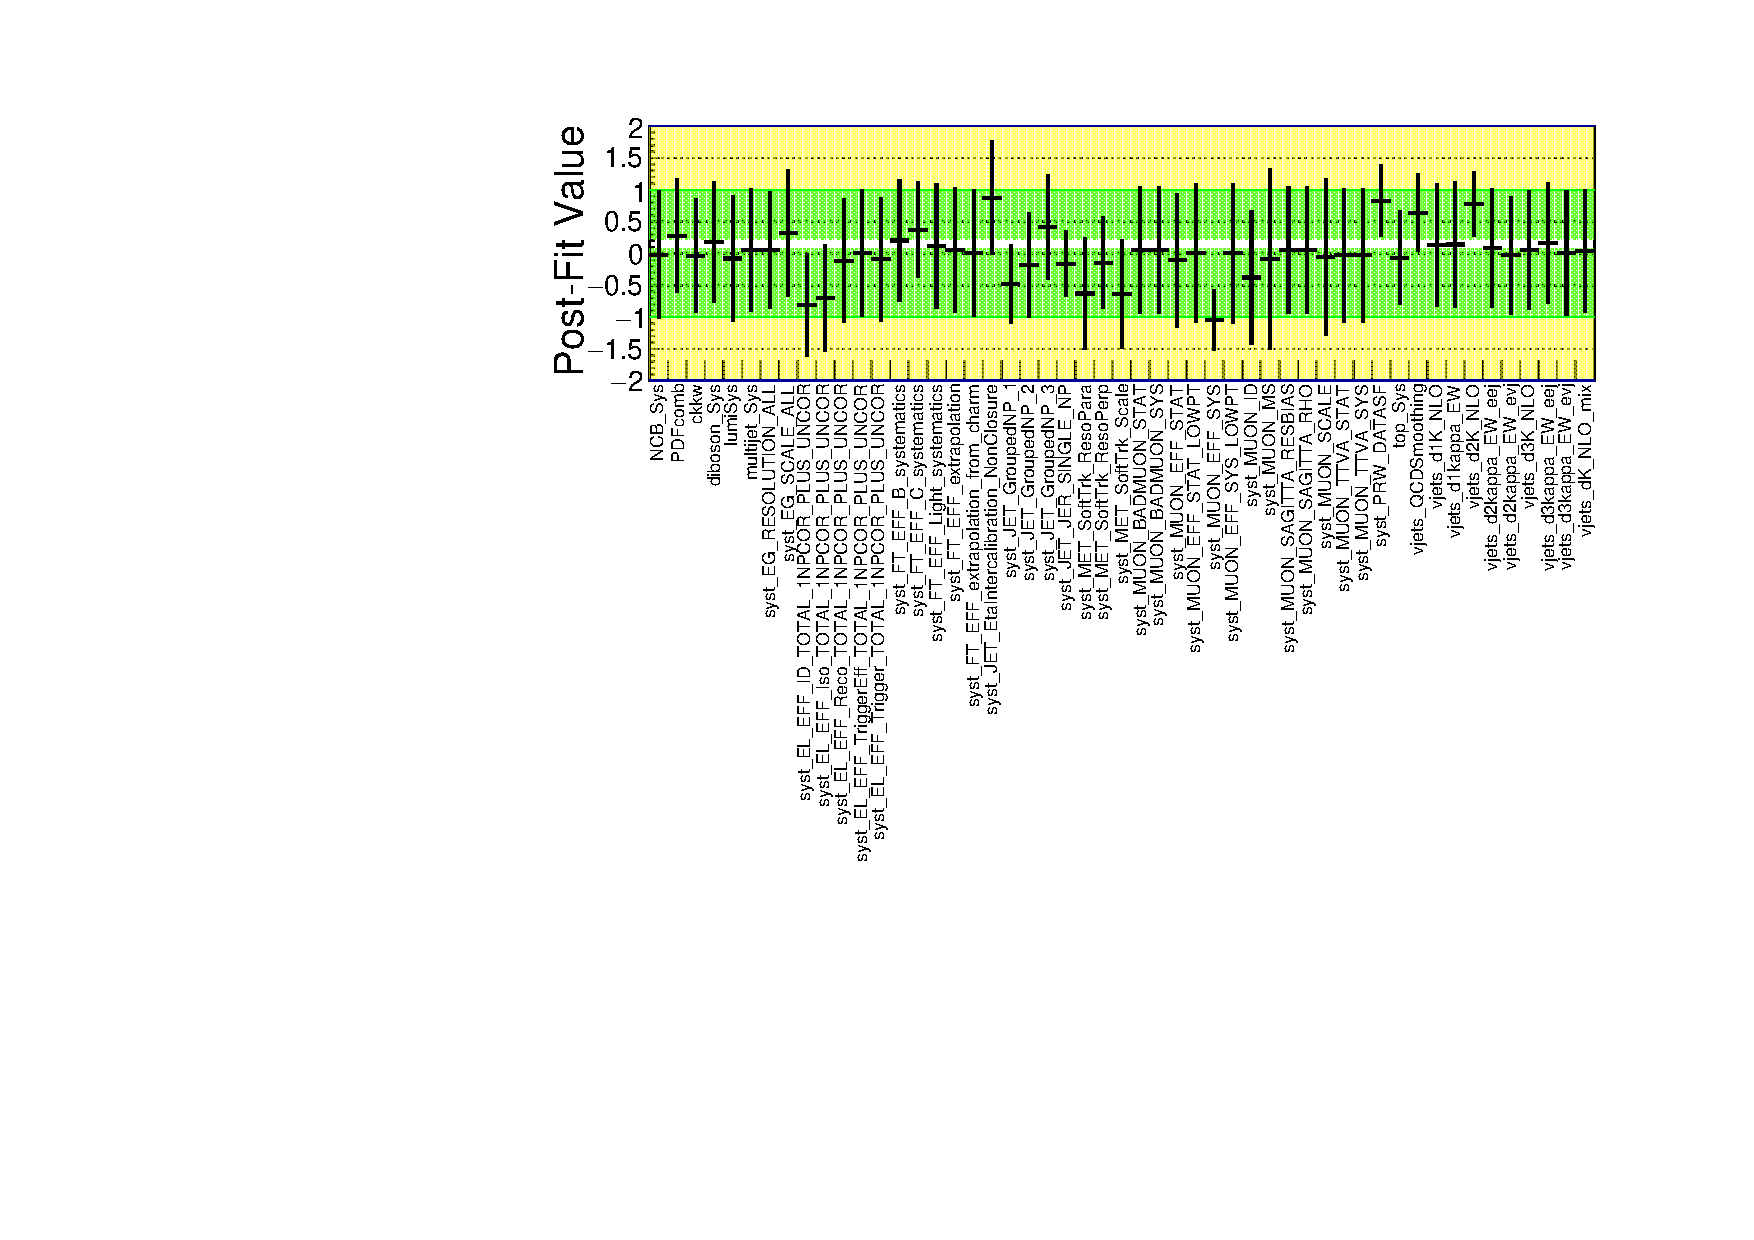
\includegraphics[width=\linewidth]{np_pull_plot}
  \caption{Values of the nuisance parameters used in the analysis after the
    control and signal region inclusive fit to the data.}
  \label{fig:np_pull}
\end{figure}
Finally \cref{fig:region_pulls} shows the comparison between data and Monte
Carlo before and after the fit for the single different regions defined in the
analysis. After the fit the agreement between data and theory expectations is
good. Since no significant excess of data compared to the predictions has been
observed, the statistical approach described in \cref{sec:stat-proc} have been
used to set 95\%~\gls{cl} model independent exclusion limits (see
\cref{sec:model-indep-limits-1}) and interpreted in terms of the ADD scenario
for large extra dimensions in \cref{sec:add-model-interpr}. The observed limits
are in general slightly worse than the expected sensitivity due to the small
excess of data compared to the Standard Model expectation as can be seen from
\cref{tab:sr_yields}.
\begin{table}[!h]
  \centering
  \begin{tabular}{lcc}
    \toprule
    \multicolumn{3}{c}{Exclusive Signal Region Yields} \\
    \midrule \midrule
    Region & Predicted & Observed \\
    \midrule
    EM1 & $111100 \pm 2300$ & 111203 \\
    EM2 & $67100 \pm 1400$ & 67475 \\
    EM3 & $33820 \pm 940$ & 35285 \\
    EM4 & $27640 \pm 610$ & 27843 \\
    EM5 & $8360 \pm 190$ & 8583 \\
    EM6 & $2825 \pm 78$ & 2975 \\
    EM7 & $1094 \pm 33$ & 1142 \\
    EM8 & $463 \pm 19$ & 512 \\
    EM9 & $213 \pm 9$ & 223 \\
    EM10 & $226 \pm 16$ & 245 \\
    \bottomrule
  \end{tabular}
  \caption{Total yields for Standard Model predictions and data in the different
    exclusive singal region selections. The statistical and systematic
    uncertainties are also quoted on the SM predictions.}
  \label{tab:sr_yields}
\end{table}
% \begin{figure}[!h]
%   \centering
%   \begin{subfigure}[t]{.48\linewidth}
%     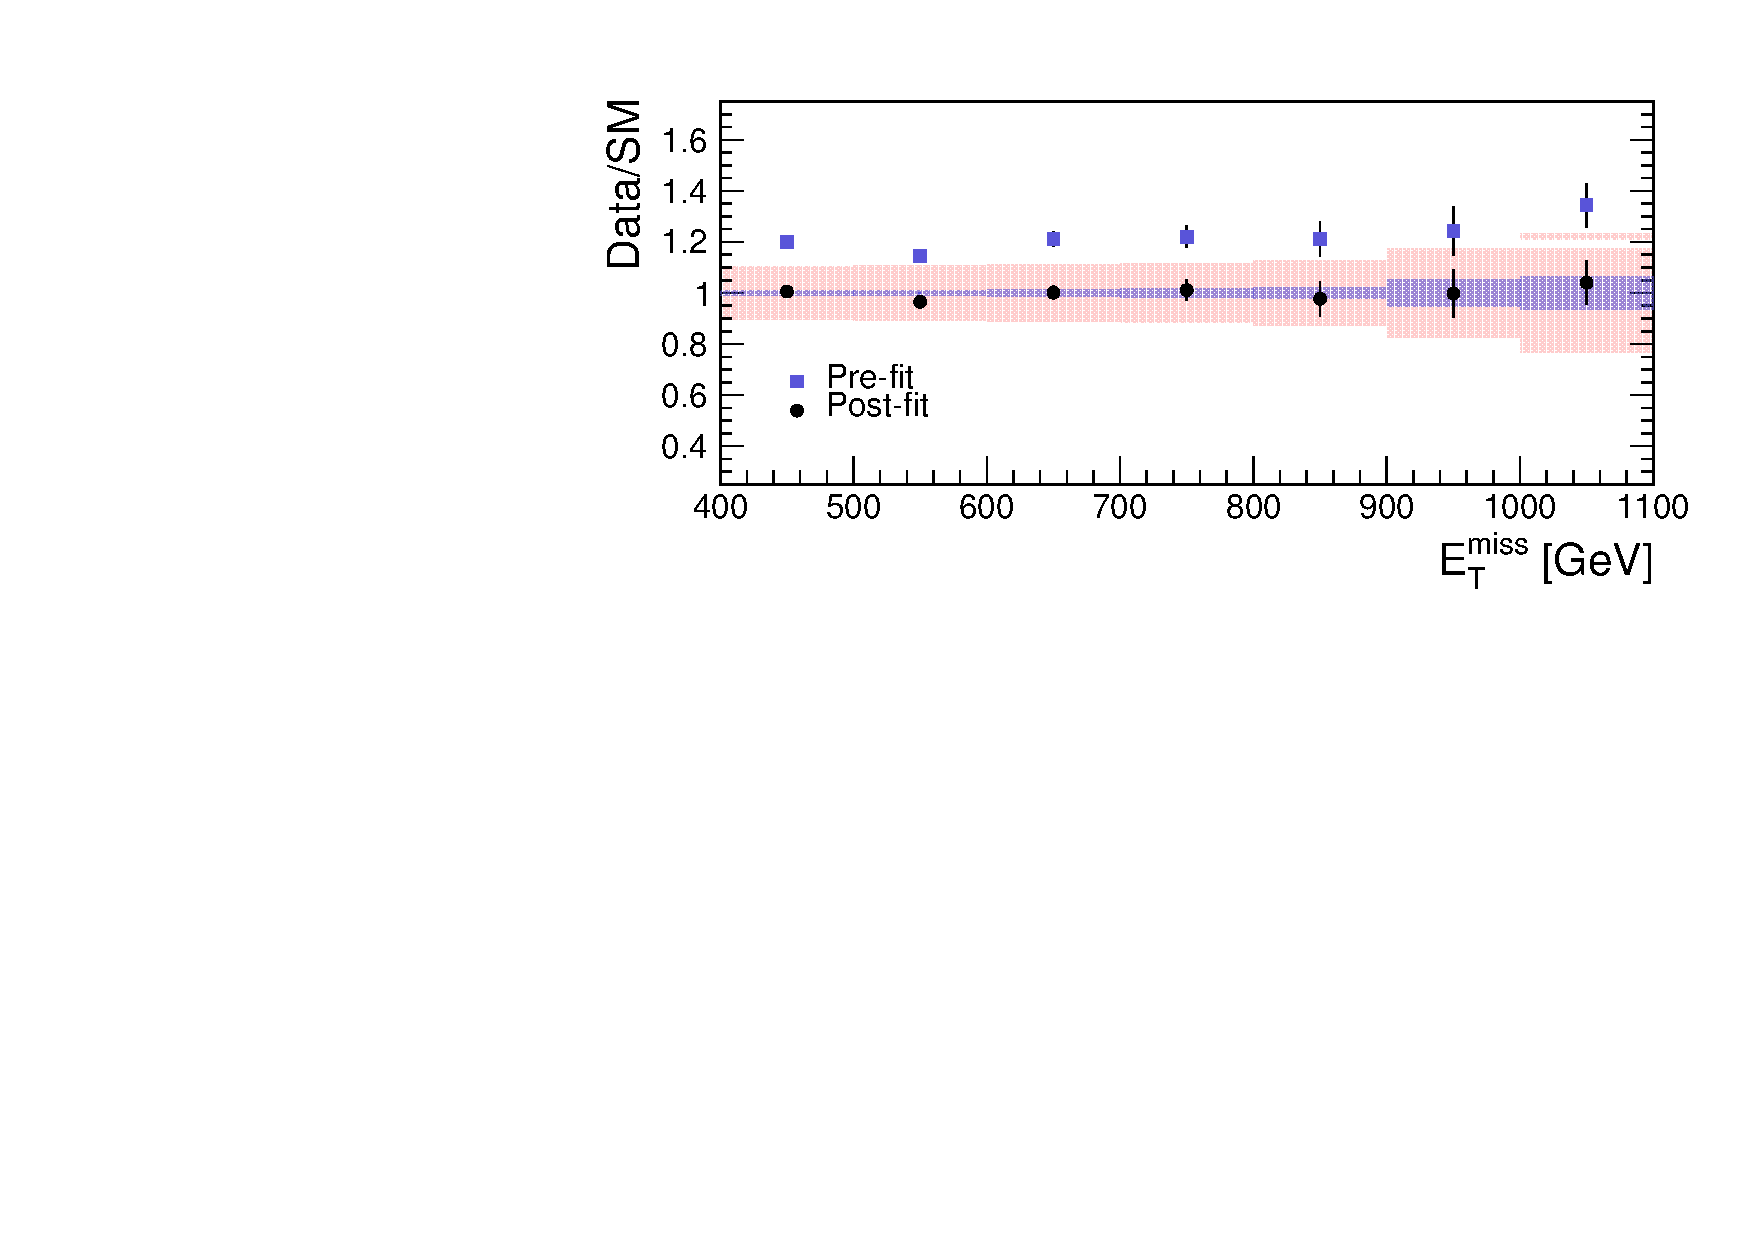
\includegraphics[width=\linewidth]{crele_pull}
%     \caption{$\crele$.}
%     \label{fig:crele_pull}
%   \end{subfigure}
%   \begin{subfigure}[t]{.48\linewidth}
%     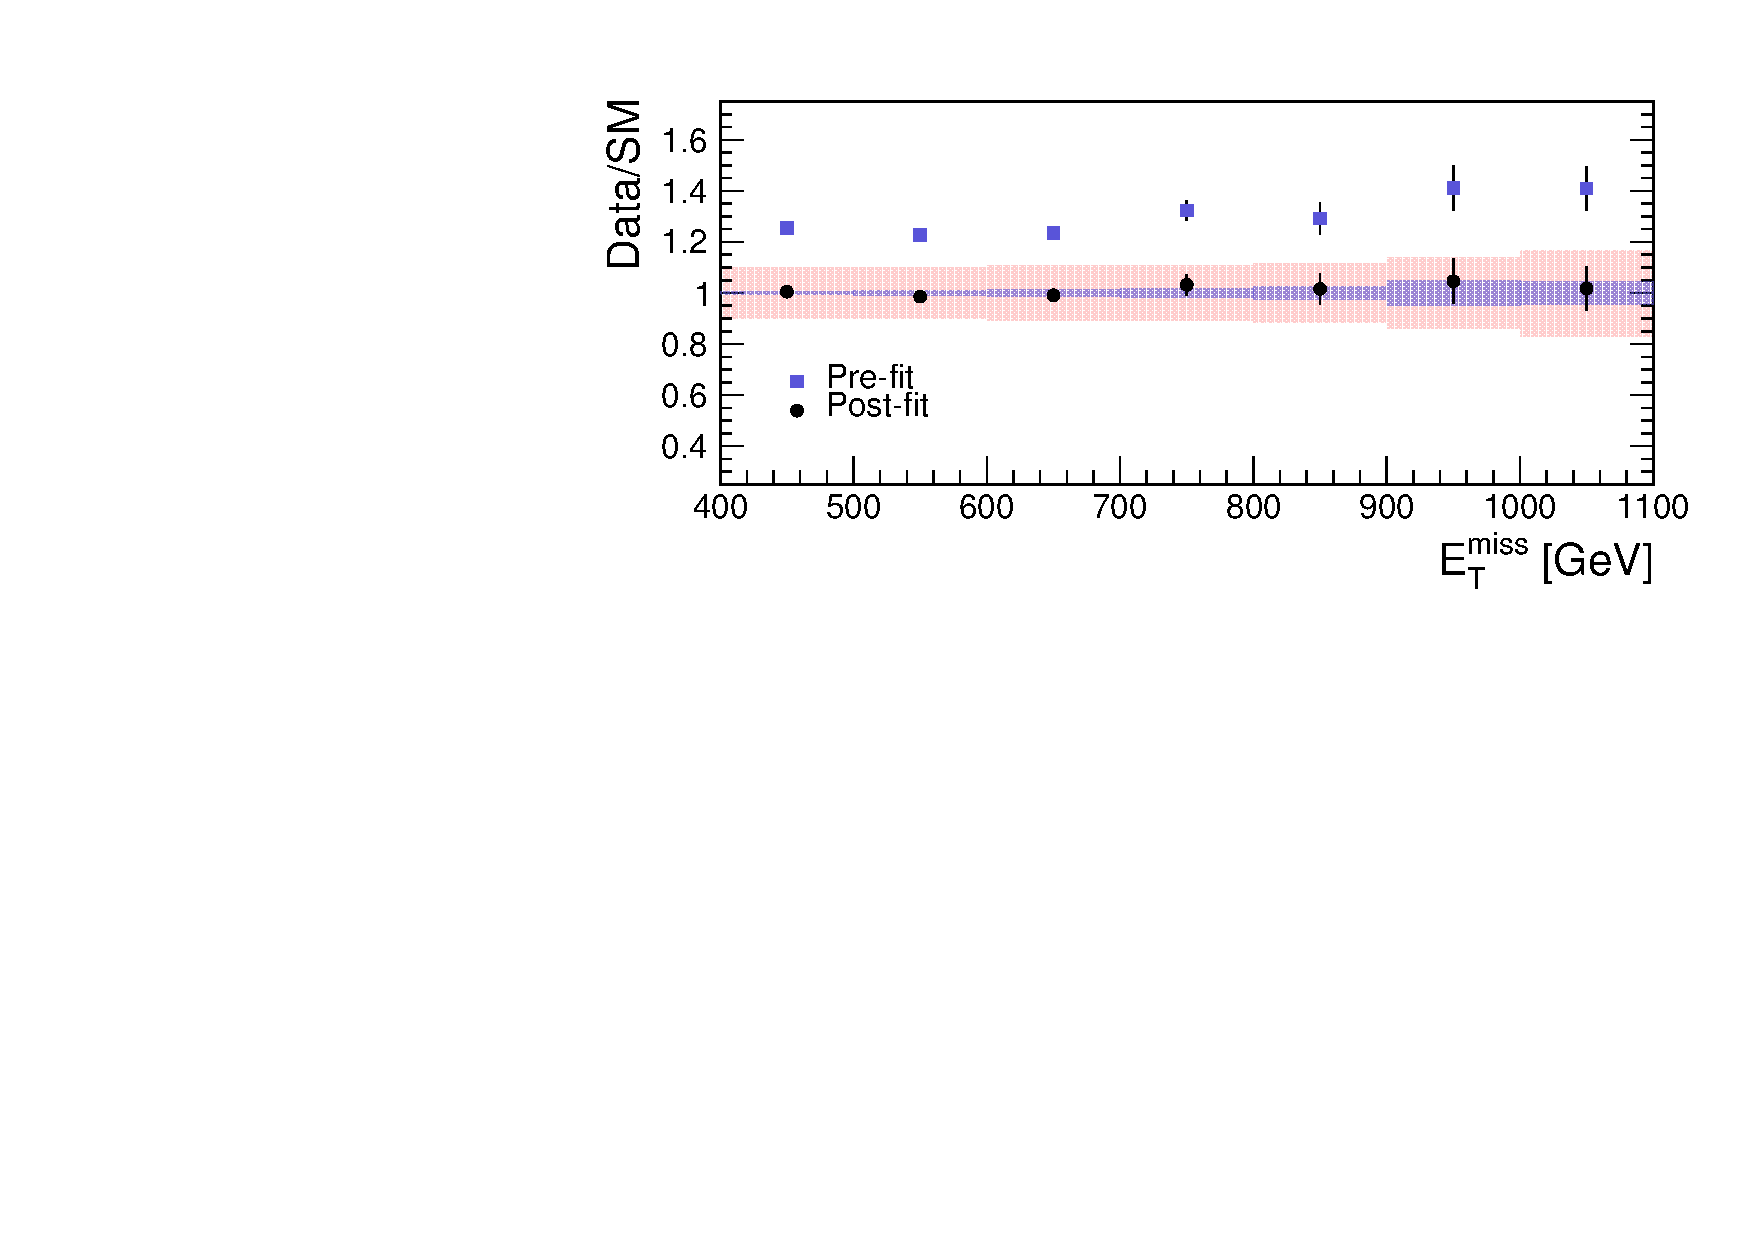
\includegraphics[width=\linewidth]{crwmn_pull}
%     \caption{$\crwmn$.}
%     \label{fig:crwnm_pull}
%   \end{subfigure}
%   \begin{subfigure}[t]{.48\linewidth}
%     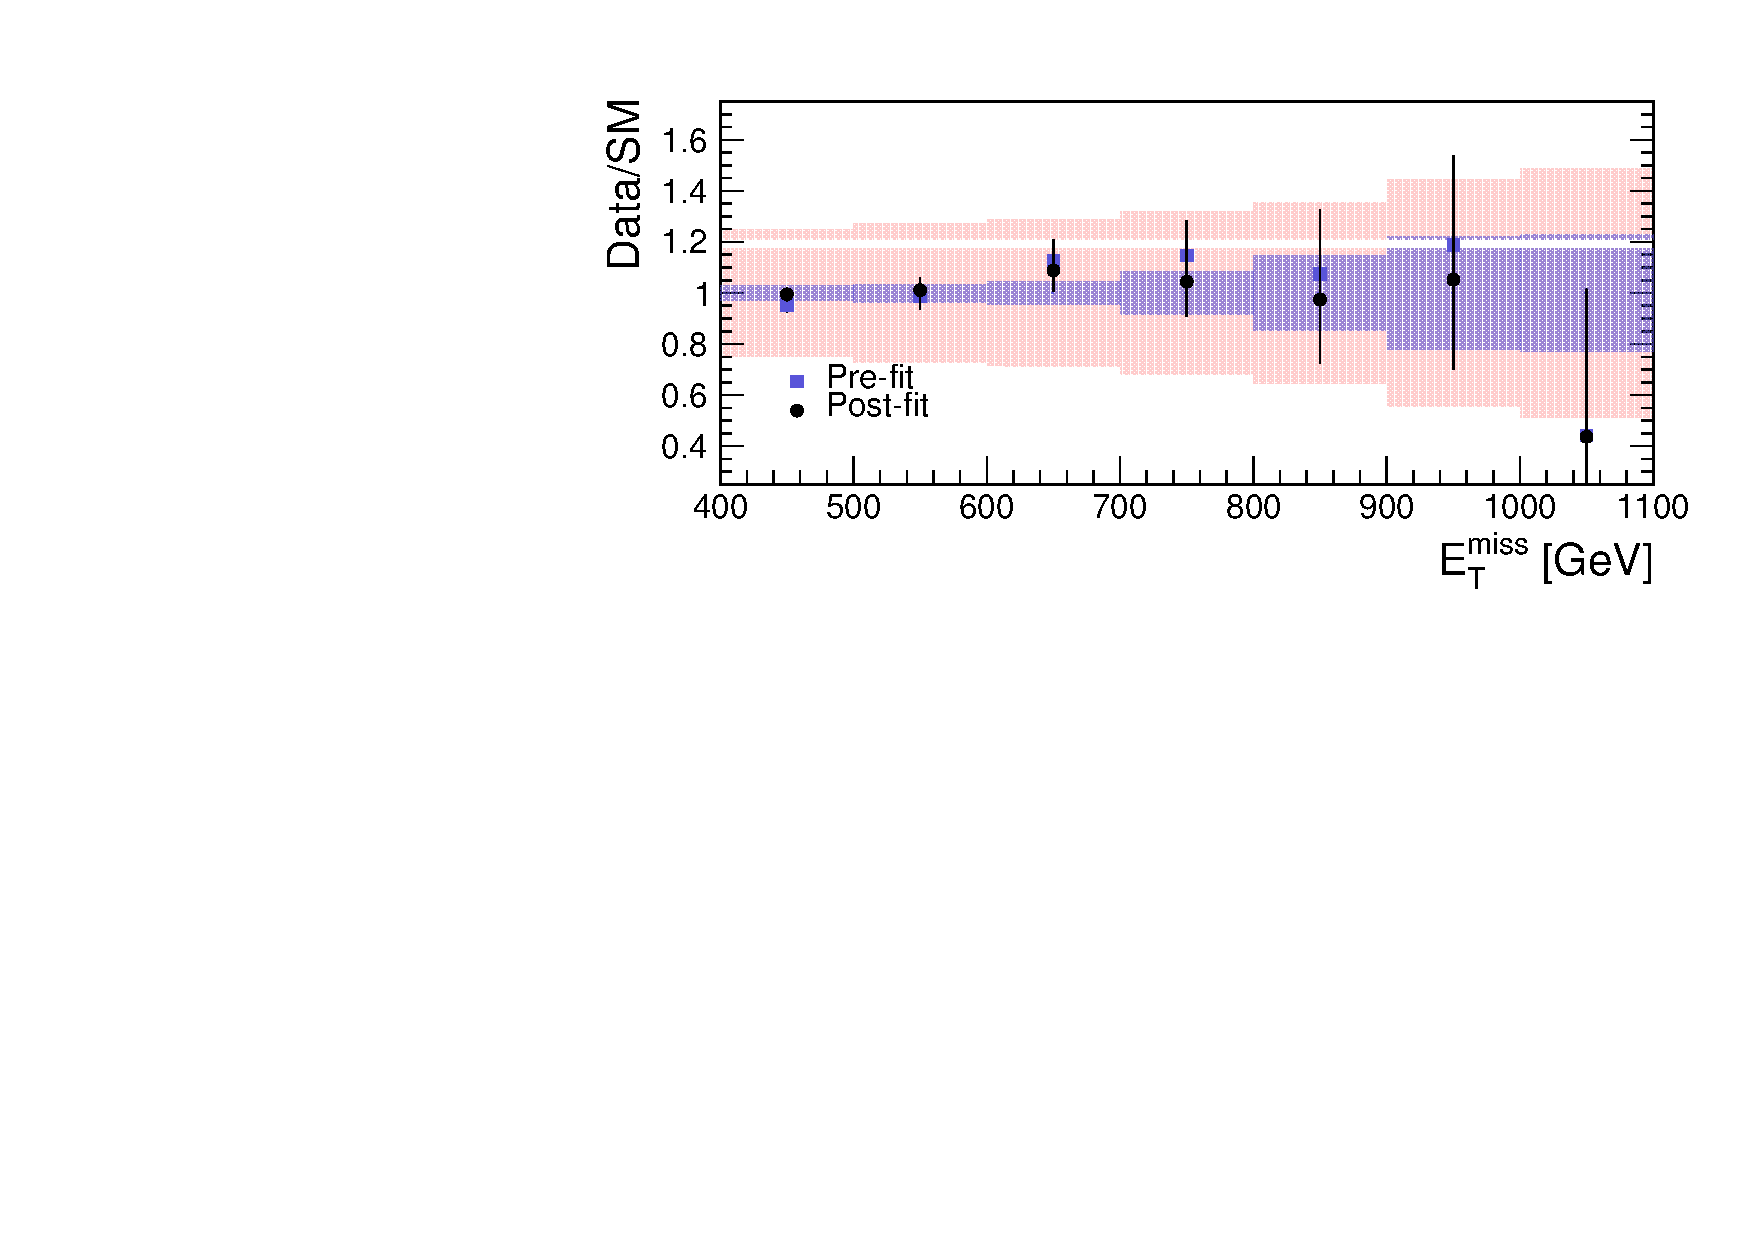
\includegraphics[width=\linewidth]{crtop_pull}
%     \caption{$\crtop$.}
%     \label{fig:crtop_pull}
%   \end{subfigure}
%     \begin{subfigure}[t]{.48\linewidth}
%     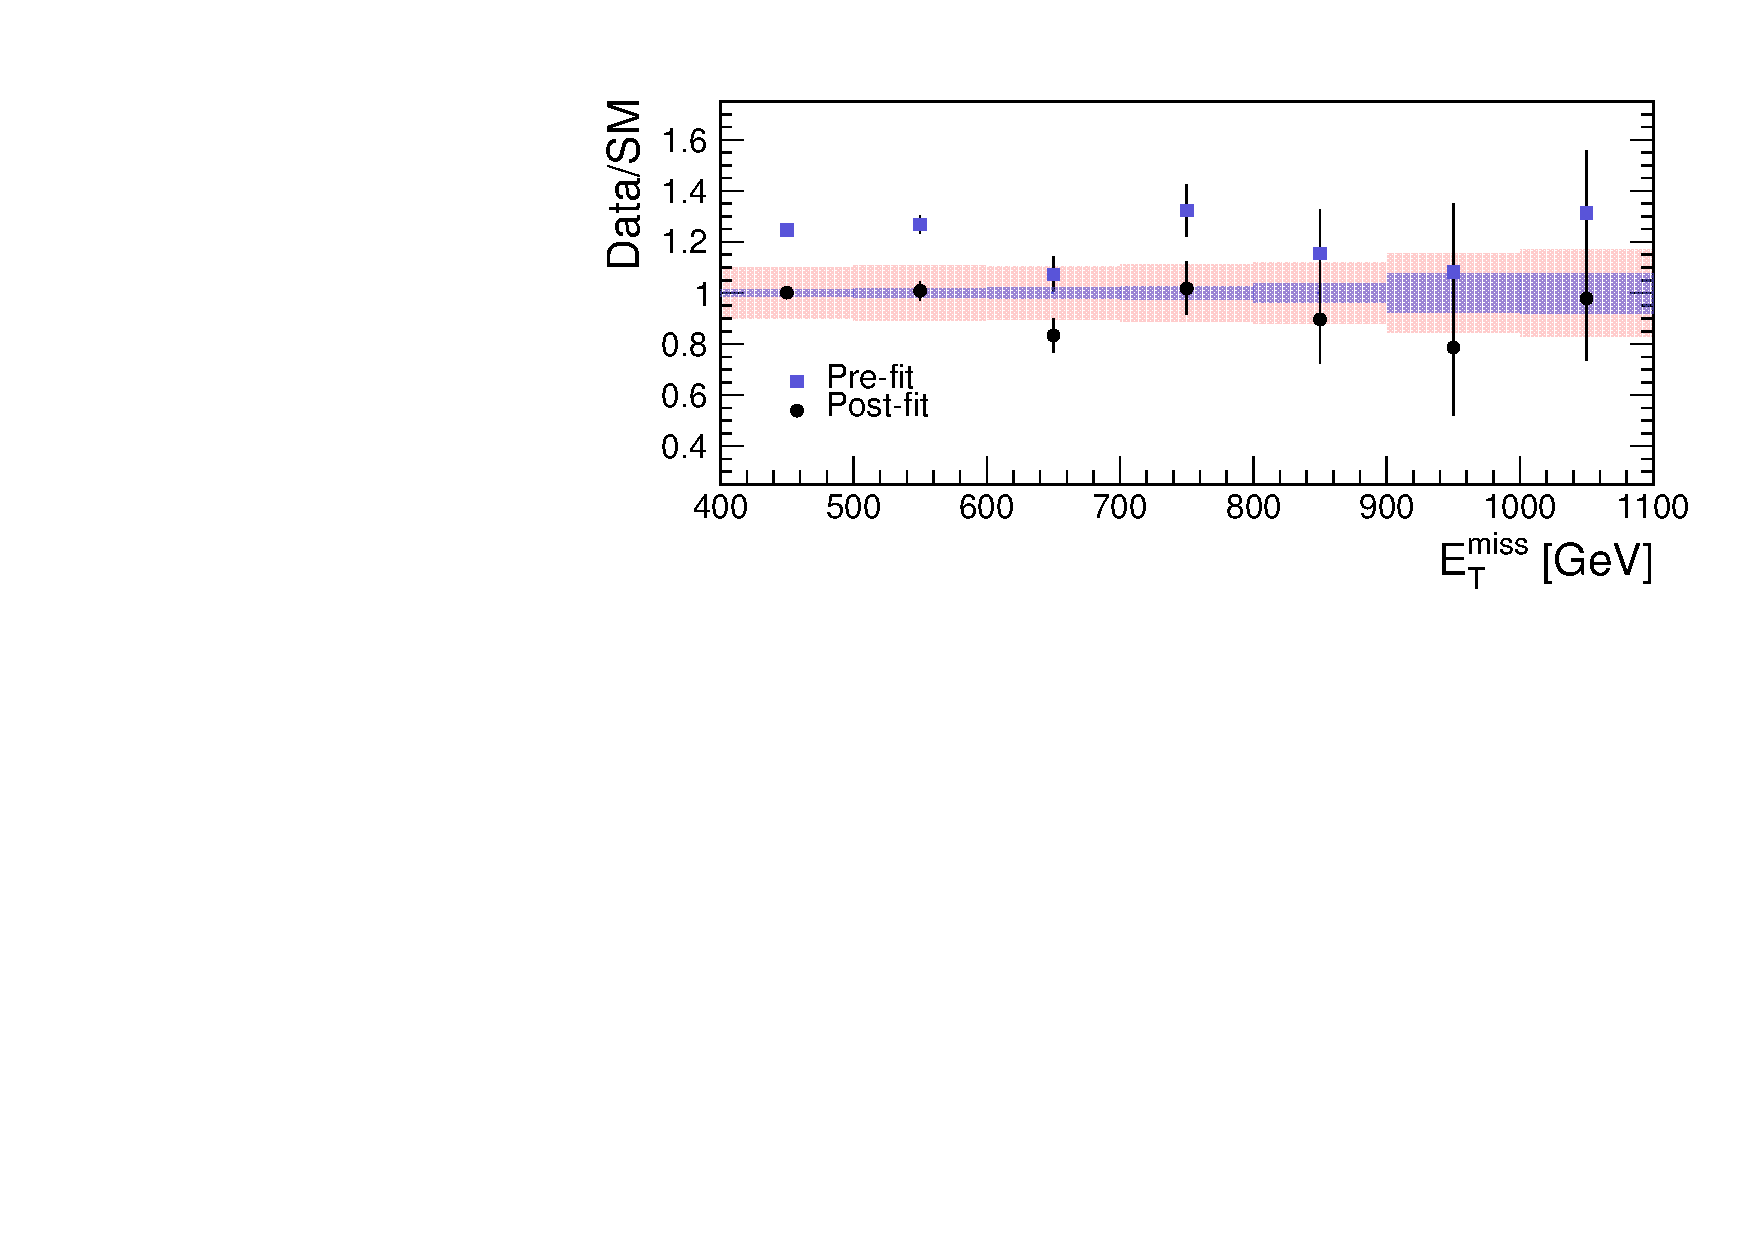
\includegraphics[width=\linewidth]{crzmm_pull}
%     \caption{$\crzmm$.}
%     \label{fig:crzmm_pull}
%   \end{subfigure}
%   \begin{subfigure}[t]{.48\linewidth}
%     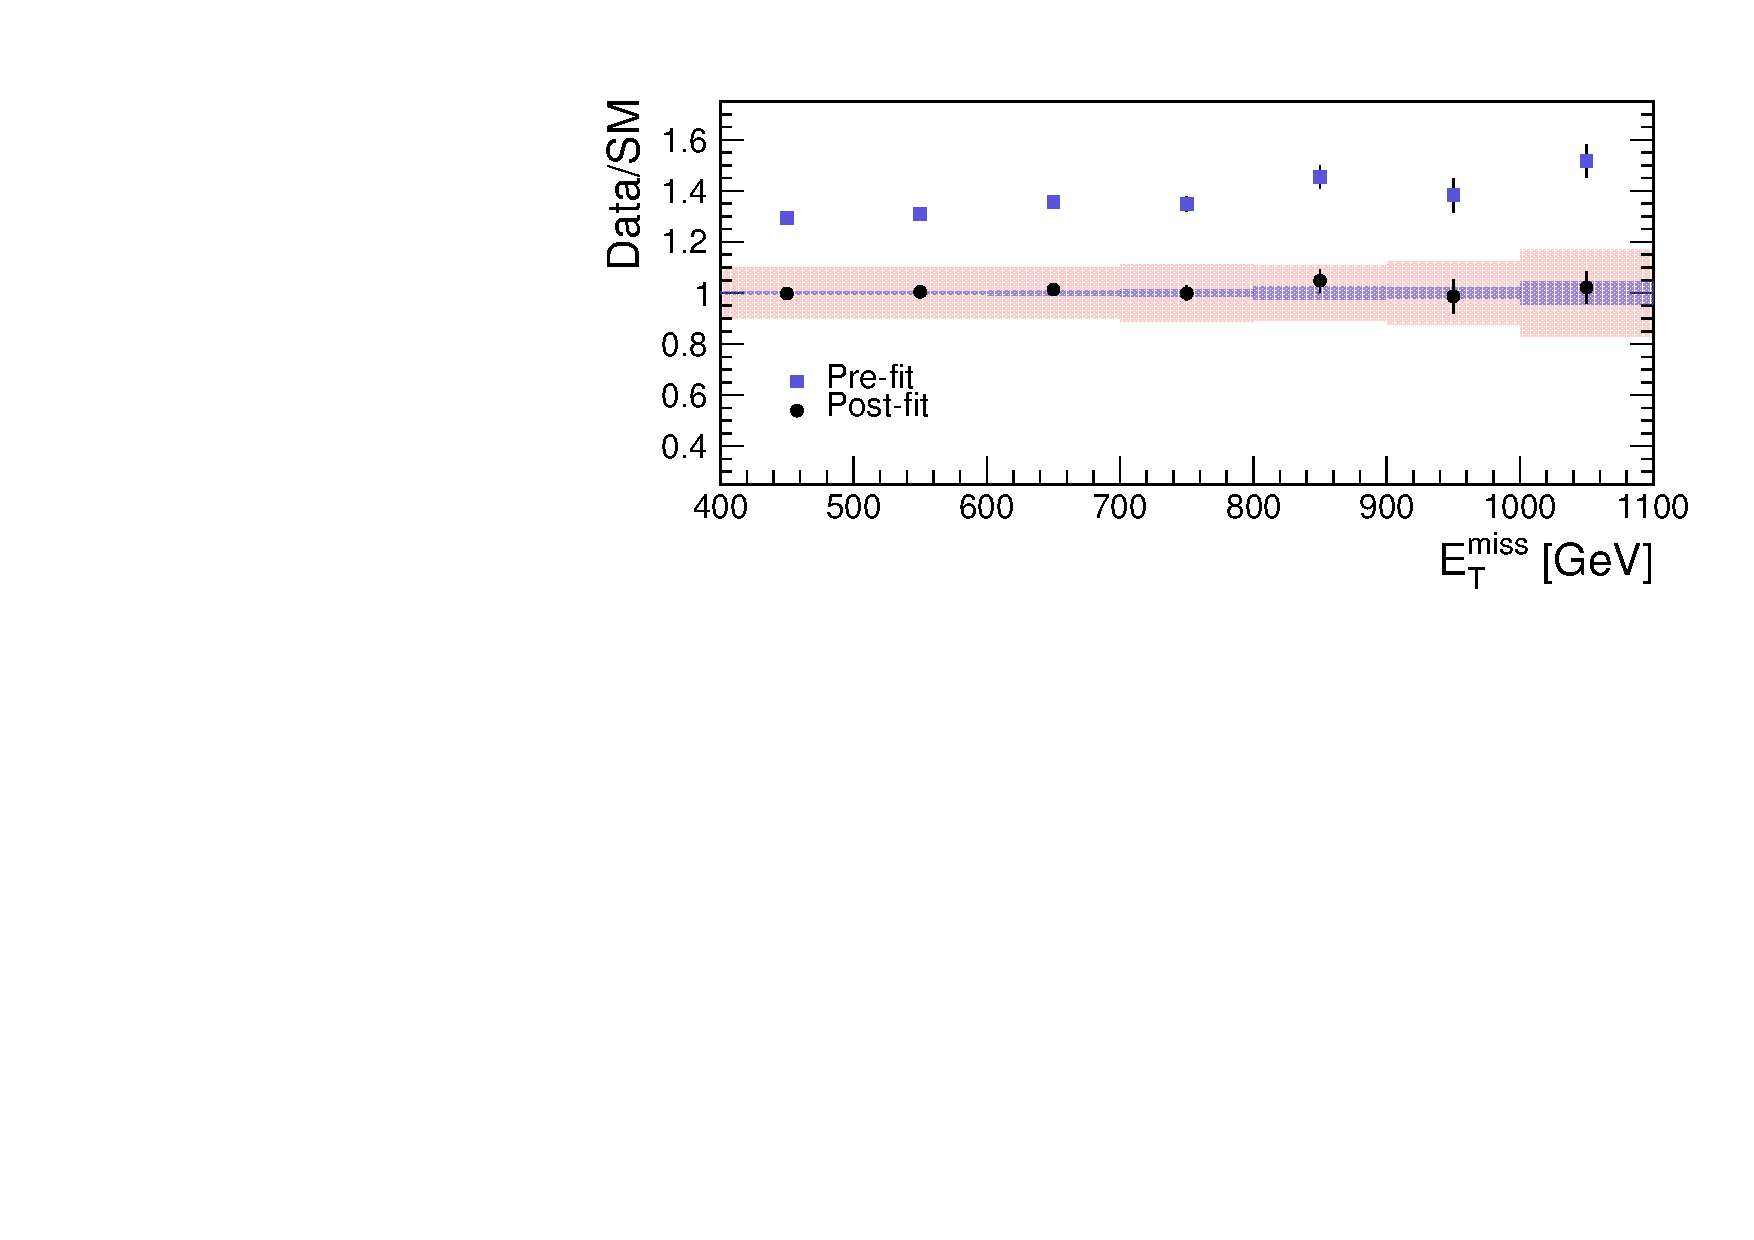
\includegraphics[width=\linewidth]{sr_pull}
%     \caption{Signal Region.}
%     \label{fig:sr_pull}
%   \end{subfigure}
%   \caption{Comparison between data and Monte Carlo before and after the fit
%     performed separately for each region. The shaded areas represent the pre and
%     post-fit total (statistic and systematic) uncertainties on the background
%     estimation.}
%   \label{fig:region_pulls}
% \end{figure}
%%% Local Variables:
%%% mode: latex
%%% TeX-master: "../search_for_DM_LED_with_ATLAS"
%%% End:
